% !TeX spellcheck = cs_CZ
%============ Kapitola: Regulační technika =========================================================
\chapter{Regulační technika}\hypertarget{tky:regulace}
\minitoc
  \section{Kde se vzala, tu se vzala, zpětná vazba}


    \begin{wrapfigure}[15]{r}{0.5\linewidth} % \ref{tky:fig_feedback005}
      \centering
      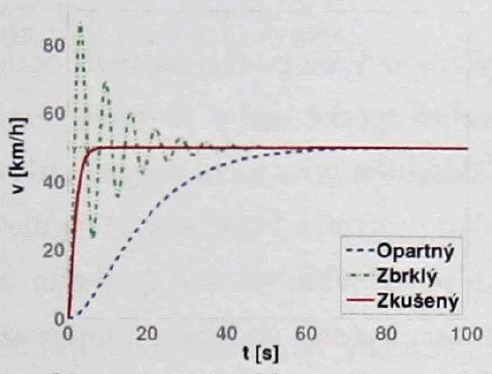
\includegraphics[width=0.9\linewidth]{Reg_smycka03.png}
      \caption{Rychlost automobilu \cite[s.~9]{Roubal2011}.}
      \label{tky:fig_feedback005}
    \end{wrapfigure}
    Protože stojící automobil má aktuální rychlost menší než žádaných \SI{50}{\km\per\hour}, 
    sešlápneme pedál plynu a automobil začne zrychlovat, což pozorujeme na tachometru. V momentě, 
    kdy je aktuální rychlost větší než žádaná, uvolníme v souladu s radami od instruktora pedál 
    plynu a rychlost automobilu začne klesat, až bude opět menší než je žádaných 
    \SI{50}{\km\per\hour}. Takto budeme dokola sešlapávat a uvolňovat pedál plynu, až dosáhneme 
    žádané rychlosti. Jistě si umíme představit, že rychlost dosažení žádané rychlosti, závisí 
    nejen na vlastnostech samotného automobilu, ale také na našich řidičských dovednostech. V 
    případě opatrného řidiče, bude rozjezd pomalý a tak se rychlost bude blížit žádané pomalu. V 
    případě zbrklého řidiče, bude rozjezd velice razantní, což povede k rychlému překročení žádané 
    rychlosti. Následné neuvážené odlehčení plynového pedálu povede k prudkému poklesu rychlosti, 
    viz zelený průběh na obr. \ref{tky:fig_feedback005}. V obou případech se nelze hovořit o dobrém 
    stylu jízdy. V prvním případě se řidič rozjíždí příliš dlouho, na vozovce představuje překážku 
    a delší dobu zbytečně unikají splodiny do ovzduší. Ve druhém případě je motor při extrémních 
    otáčkách příliš hlučný, dochází k nekvalitnímu spalování a opět k úniku škodlivin do ovzduší. 
    Styl jízdy nepůsobí příliš uklidňujícím dojmem na ostatní řidiče a účastníky silničního provozu.
    
    Pro kvalitní dosažení žádané hodnoty rychlosti je třeba znát \emph{dynamický model} automobilu. 
    Tedy nejen sešlápni pedál plynu, uvolni pedál plynu, což můžeme považovat za \emph{statický 
    model} (v čase neproměnný), ale právě popis jak rychle se automobil rozjíždí, když takovým a 
    takovým způsobem sešlápneme pedál plynu. V regulační technice budeme mít dynamický model 
    systému tvořený převážně diferenciálními (pohybovými) rovnicemi. Modelováním reálných 
    dynamických systémů se budeme zabývat v kapitole \ref{TKY:sec002}. Procesu získávání modelu 
    fyzikální reality říkáme \textbf{identifikace systému} a v našem příkladě s automobilem ji 
    vlastně provádíme tím, že se učíme jezdit. Na identifikaci dynamických systémů a její praktické 
    aspekty se zaměříme v kapitole \ref{TKY:sec003}.

    V momentě, kdy máme dynamický model systému, přichází další krok a to je vlastní \textbf{návrh 
    regulátoru}, neboli návrh algoritmu řízení. V momentě, kdy už řidič ví, jak automobil reaguje 
    na změny vstupu, může dosáhnout žádané výstupní veličiny mnohem lépe, viz obr. 
    \ref{tky:fig_feedback003}. Na rozdíl od řidiče, jenž má naučený regulátor ve své hlavě, v 
    regulační technice budeme využívat různé matematické metody. Možná nás nyní napadne, že model 
    automobilu není pouze závislost mezi pedálem plynu a rychlostí automobilu. Chování automobilu 
    ovlivňuje samozřejmě mnoho dalších okolností, jako je přilnavost pneumatik k povrchu vozovky, 
    vlhkost vozovky a podobně. V momentě, kdy například zaprší, může řidič se svým regulátorem v 
    zatáčce opustit vozovku, pokud jsme příliš agresivní, protože se reálný systém změnil, ale jeho 
    model tuto informaci nemá. Opět tedy musíme vzít v potaz nové faktory a provést identifikaci 
    znovu, a tím získat více informací o chování systému za těchto podmínek. Pak bude řidič schopen 
    jezdit bezpečně za sucha i za mokra a tak dále. V regulační technice je vždy přesnost modelu 
    zásadní otázkou. Na jedné straně požadujeme model systému co nejpřesnější, abychom byli schopni 
    navrhnout dobrý regulátor. Na druhé straně se pro příliš složitý model navrhuje regulátor 
    obtížněji. Proto vždy musíme zvolit jistý kompromis tak, aby v modelu byly zahrnuty všechny 
    podstatné vlastnosti systému.

    Tím ale regulace nekončí. Například cena paliva není již dnes zanedbatelná, a tak budeme třeba 
    chtít jezdit s minimální spotřebou. To znamená, že musíme zjistit závislost spotřeby paliva na 
    stylu jízdy. Poté musíme definovat nějaké kritérium kvality regulace obsahující tuto závislost 
    a podle něho navrhnout nový regulátor, který zajistí minimální spotřebu paliva.  Problémů v 
    oblasti řízení je samozřejmě mnohem a mnohem víc  (odhadování a filtrace, robustní řízení a 
    nelineární systémy). My však zde tento příklad ukončíme s konstatováním, že v regulační 
    technice jde především o tyto body:
    \begin{itemize}\addtolength{\itemsep}{-0.5\baselineskip}
      \item určení vstupů a výstupů systému,
      \item identifikace systému (určení chování systému na výstupech pro nějaké chování vstupů),
      \item návrh regulátoru pro zajištění požadovaných vlastností; testování regulátoru na 
            počítači; aplikace regulátoru na reálném systému; případně návrh v nějakém smyslu 
            optimálního regulátoru.
    \end{itemize}
    
  \section{Regulační smyčka a základní typy PID regulátorů}\label{TKY:sec001}
    \begin{wrapfigure}[6]{r}{0.5\linewidth} % \ref{tky:fig_feedback003}
      \centering
      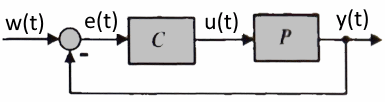
\includegraphics[width=0.9\linewidth]{Reg_smycka01.png}
      \caption{Regulační smyčka \cite[s.~215]{Roubal2011}.}
      \label{tky:fig_feedback003}
    \end{wrapfigure}
    Ve snaze řídit systémy rozeznáváme dva hlavní způsoby řízení:
      \begin{itemize}
        \item \textbf{přímovazební},
        \item \textbf{zpětnovazební}.
      \end{itemize}
    \textbf{Přímovazební řízení} (\emph{řízení v otevřené smyčce}), zvané také jako ovládání, má 
    jednodušší zapojení, ovšem jeho nevýhodou je nemožnost reagovat na poruchy či změny soustavy a 
    my se jím zde dále zabývat nebudeme. Naproti tomu \textbf{zpětnovazební řízení} (\emph{řízení v 
    uzavřené smyčce}), obecně označované jako \textbf{regulace}, porovnává \emph{výstup soustavy} 
    \(y(t)\) s \emph{požadovaným výstupem} \(w(t)\), a podle této informace generuje \emph{akční 
    zásah} \(u(t)\) do řízeného systému. Regulace nám tak dává mimo jiné možnost 
    \emph{stabilizovat} nestabilní soustavy.
    
    V této kapitole se budeme věnovat regulaci, regulační smyčce a základním typů regulátorů. 
    Ukážeme si dvě základní zapojení regulačních smyček a zavedeme jednotné názvosloví, zejména 
    proto, že toto názvosloví není ustálené. Vysvětlíme si některé míry kvality řízení a ukážeme 
    názorně na příkladech vlastnosti základních \textbf{PID regulátorů}. Zvláštní pozornost bude 
    věnována filtraci derivační složky u tohoto regulátoru. Konkrétní způsoby návrhu regulátorů si 
    ukážeme v následujících kapitolách.
    
  
  \section{Modelování fyzikálních systémů}\label{TKY:sec002}
    Doposud jsme se v předešlých kapitolách zabývali různými nástroji, jak popisovat dynamické 
    chování systémů. Šlo spíše o teorii rozdělenou do kapitol bez větších souvislostí. V této kar 
    kapitole bychom chtěli ukázat použití těchto teoretických poznatků na konkrétních příkladech 
    fyzikálních systémů. Odvodíme zde několik matematických modelů fyzikálních systémů a připravíme 
    k těmto modelům simulinkové soubory s virtuální realitou pro Matlab (The Mathworks, 2009).
    
  \section{Identifikace systémů}\label{TKY:sec003}
    
%---------------------------------------------------------------------------------------------------
\printbibliography[title={Seznam literatury}, heading=subbibliography]
\addcontentsline{toc}{section}{Seznam literatury}